\section{Chapter 7 Research Methodology}

\subsection{7.1 Introduction}

This chapter presents the research methodology adopted for the design, development, and evaluation of the proposed CloudSentinel AI framework. The methodology provides a systematic approach for developing a context-aware cloud security solution capable of identifying cloud misconfigurations, modeling resource relationships, generating attack paths, assessing contextual risks, and producing explainable security recommendations. The proposed methodology combines cloud asset collection, graph-based data modeling, rule-based security assessment, contextual risk analysis, and Artificial Intelligence into a unified research framework. Each phase of the methodology builds upon the results of the previous phase, ensuring that the final system provides an accurate and comprehensive assessment of cloud security risks. The complete research methodology is illustrated in Figure 7.1, which depicts the sequential phases involved in the development and evaluation of CloudSentinel AI.

\begin{figure}[H]
\centering
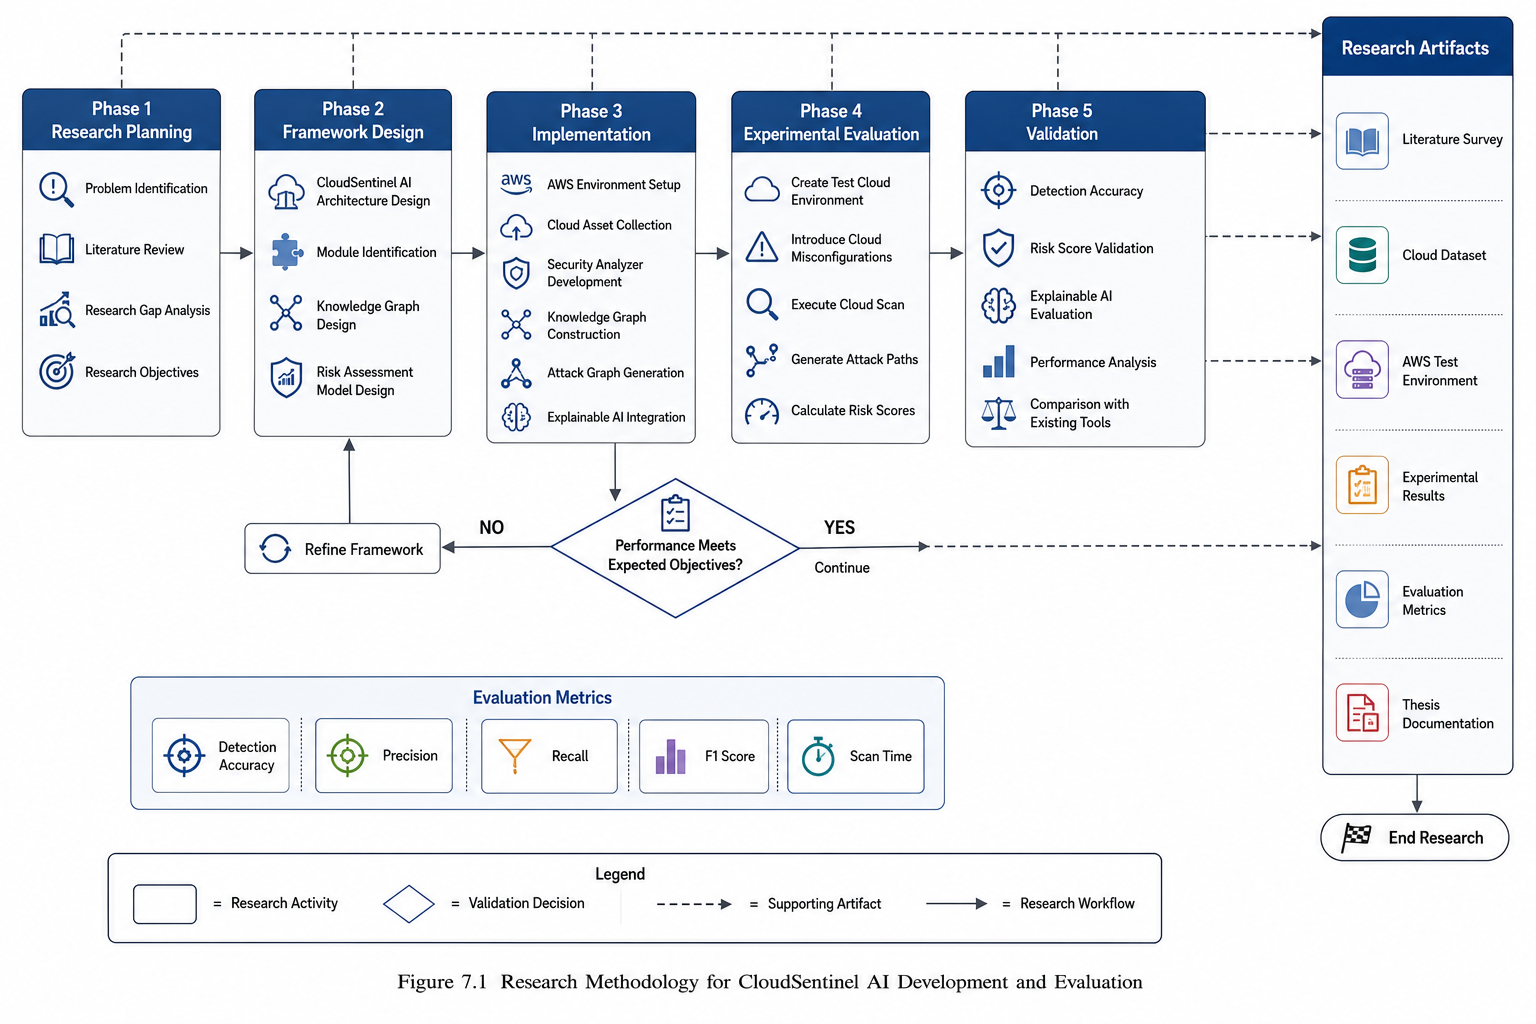
\includegraphics[width=0.9\textwidth,height=\textheight]{figures/image-7.1.png}
\caption{Research Methodology Workflow.}\label{fig:7_1}
\end{figure}

\subsection{7.2 Research Design}

The proposed research follows a Design Science Research (DSR) methodology \cite{hevner2004design}. Design Science Research is widely adopted in information systems and cybersecurity research because it focuses on creating and evaluating innovative artifacts that solve real-world problems. In this research, the primary artifact is the CloudSentinel AI framework, which is designed to address the limitations of existing Cloud Security Posture Management (CSPM) solutions. The research process consists of the following phases:

\begin{enumerate}
\def\labelenumi{\arabic{enumi}.}
\tightlist
\item
  Problem Identification\\
\item
  Requirement Analysis\\
\item
  Framework Design\\
\item
  System Development\\
\item
  Experimental Evaluation\\
\item
  Performance Analysis\\
\item
  Conclusion and Future Improvements
\end{enumerate}

Each phase contributes to the iterative refinement of the proposed framework, ensuring that the final solution addresses both practical cloud security challenges and the identified research gaps.

\subsection{7.3 Research Workflow}

The overall workflow of the proposed research consists of six major stages.\\
\textbf{Phase 1 -- Cloud Environment Preparation}\\
An AWS environment will be configured to simulate real-world cloud infrastructure. The environment will contain multiple AWS services, including EC2, IAM, S3, VPC, RDS, Security Groups, and CloudTrail. The cloud environment will intentionally include both secure and insecure configurations to evaluate the effectiveness of the proposed framework.\\
\textbf{Phase 2 -- Cloud Asset Collection}\\
The Cloud Asset Collector will communicate with AWS APIs to retrieve metadata describing cloud resources and their security configurations.\\
\textbf{Inputs:}

\begin{itemize}
\tightlist
\item
  AWS Credentials\\
\item
  AWS SDK (Boto3)\\
\item
  AWS Service APIs
\end{itemize}

\textbf{Processing:}

\begin{itemize}
\tightlist
\item
  Authenticate with AWS.\\
\item
  Discover cloud resources.\\
\item
  Retrieve metadata.\\
\item
  Store collected information.
\end{itemize}

\textbf{Outputs:}

\begin{itemize}
\tightlist
\item
  Cloud Asset Inventory\\
\item
  Configuration Metadata
\end{itemize}

\textbf{Phase 3 -- Configuration Assessment}\\
The collected cloud resources will be analyzed against predefined security policies derived from established cloud security frameworks.\\
\textbf{Inputs:}

\begin{itemize}
\tightlist
\item
  Cloud Resource Metadata\\
\item
  Security Policies\\
\item
  Compliance Rules
\end{itemize}

\textbf{Processing:}

\begin{itemize}
\tightlist
\item
  Evaluate configurations.\\
\item
  Detect policy violations.\\
\item
  Assign initial severity.
\end{itemize}

\textbf{Outputs:}

\begin{itemize}
\tightlist
\item
  Misconfiguration Report\\
\item
  Initial Security Findings
\end{itemize}

\textbf{Phase 4 -- Knowledge Graph Construction}\\
The validated cloud resources will be transformed into a graph representation.\\
\textbf{Inputs:}

\begin{itemize}
\tightlist
\item
  Cloud Resources\\
\item
  IAM Relationships\\
\item
  Network Topology\\
\item
  Storage Relationships
\end{itemize}

\textbf{Processing:}

\begin{itemize}
\tightlist
\item
  Create graph nodes.\\
\item
  Create graph edges.\\
\item
  Store graph.
\end{itemize}

\textbf{Outputs:}

\begin{itemize}
\tightlist
\item
  Knowledge Graph\\
\item
  Relationship Database
\end{itemize}

\textbf{Phase 5 -- Attack Path Generation}\\
The Knowledge Graph will be analyzed to identify realistic attack paths.\\
\textbf{Inputs:}

\begin{itemize}
\tightlist
\item
  Knowledge Graph
\end{itemize}

\textbf{Processing:}

\begin{itemize}
\tightlist
\item
  Traverse graph.\\
\item
  Identify exploitable paths.\\
\item
  Calculate attack chains.
\end{itemize}

\textbf{Outputs:}

\begin{itemize}
\tightlist
\item
  Attack Graph\\
\item
  Exploitation Paths
\end{itemize}

\textbf{Phase 6 -- Context-Aware Risk Assessment}\\
The identified attack paths will be evaluated using contextual information to generate dynamic risk scores.\\
\textbf{Inputs:}

\begin{itemize}
\tightlist
\item
  Attack Graph\\
\item
  Asset Criticality\\
\item
  Network Exposure\\
\item
  Identity Permissions
\end{itemize}

\textbf{Processing:}

\begin{itemize}
\tightlist
\item
  Analyze context.\\
\item
  Calculate dynamic risk.\\
\item
  Prioritize findings.
\end{itemize}

\textbf{Outputs:}

\begin{itemize}
\tightlist
\item
  Risk Score\\
\item
  Prioritized Findings
\end{itemize}

\textbf{Phase 7 -- Explainable AI Analysis}\\
The Explainable AI module converts technical findings into natural-language security recommendations.\\
\textbf{Inputs:}

\begin{itemize}
\tightlist
\item
  Attack Paths\\
\item
  Risk Scores
\end{itemize}

\textbf{Processing:}

\begin{itemize}
\tightlist
\item
  Generate explanation.\\
\item
  Produce remediation recommendations.
\end{itemize}

\textbf{Outputs:}

\begin{itemize}
\tightlist
\item
  Human-readable Security Report\\
\item
  AI Recommendations
\end{itemize}

\subsection{7.4 Research Environment}

The proposed framework will initially be developed and evaluated using Amazon Web Services (AWS).

\begin{itemize}
\tightlist
\item
  Cloud Platform: Amazon Web Services (AWS)\\
\item
  Programming Language: Python\\
\item
  Backend Framework: FastAPI\\
\item
  Graph Processing: NetworkX\\
\item
  Graph Database (Future Extension): Neo4j\\
\item
  Database: PostgreSQL\\
\item
  Dashboard: React.js\\
\item
  AI Integration: Large Language Model (LLM)\\
\item
  Version Control: Git and GitHub\\
\item
  Deployment: Docker
\end{itemize}

\subsection{7.5 Dataset}

Unlike traditional machine learning research, CloudSentinel AI does not rely on a static benchmark dataset. Instead, the framework generates its dataset dynamically by collecting metadata directly from cloud resources deployed within the AWS environment. The dataset consists of:

\begin{itemize}
\tightlist
\item
  IAM Policies\\
\item
  EC2 Configurations\\
\item
  Security Groups\\
\item
  VPC Configuration\\
\item
  S3 Bucket Policies\\
\item
  CloudTrail Logs\\
\item
  RDS Configuration\\
\item
  Encryption Settings
\end{itemize}

This approach ensures that the evaluation reflects realistic cloud environments rather than synthetic benchmark datasets.

\subsection{7.6 Evaluation Metrics}

The effectiveness of the proposed framework will be evaluated using multiple qualitative and quantitative metrics.\\
\textbf{Security Metrics:}

\begin{itemize}
\tightlist
\item
  Number of detected misconfigurations\\
\item
  Number of generated attack paths\\
\item
  Critical attack paths identified\\
\item
  False positive rate\\
\item
  False negative rate
\end{itemize}

\textbf{Performance Metrics:}

\begin{itemize}
\tightlist
\item
  Asset collection time\\
\item
  Graph construction time\\
\item
  Risk calculation time\\
\item
  Total assessment time
\end{itemize}

\textbf{AI Evaluation:}

\begin{itemize}
\tightlist
\item
  Explanation quality\\
\item
  Recommendation relevance\\
\item
  Analyst usability\\
\item
  Interpretability
\end{itemize}

\textbf{System Metrics:}

\begin{itemize}
\tightlist
\item
  CPU utilization\\
\item
  Memory usage\\
\item
  Scalability\\
\item
  API response time
\end{itemize}

\subsection{7.7 Research Validation}

To validate the effectiveness of CloudSentinel AI, the proposed framework will be compared against existing cloud security solutions. The comparison will focus on the following criteria:

\begin{itemize}
\tightlist
\item
  Cloud misconfiguration detection\\
\item
  Attack path identification\\
\item
  Context-aware risk analysis\\
\item
  Explainable AI support\\
\item
  Risk prioritization\\
\item
  Graph-based analysis\\
\item
  Analyst usability
\end{itemize}

Experimental results obtained from the proposed framework will be analyzed against these criteria to determine its effectiveness in improving cloud security assessment.

\subsection{7.8 Ethical Considerations}

All experiments conducted as part of this research will be performed within controlled cloud environments owned or authorized for research purposes. No unauthorized access to third-party cloud environments will be attempted. The framework is intended solely for defensive cybersecurity research, cloud security assessment, and educational purposes. The research complies with responsible disclosure principles and aims to improve cloud security practices without introducing risks to production systems.

\subsection{7.9 Chapter Summary}

This chapter presented the research methodology adopted for the development and evaluation of the proposed CloudSentinel AI framework. The methodology follows a structured Design Science Research approach, beginning with cloud environment preparation and progressing through cloud asset collection, configuration assessment, knowledge graph construction, attack path generation, contextual risk assessment, Explainable AI integration, and experimental validation. The methodology establishes a clear roadmap for implementing and evaluating the proposed framework while ensuring that each phase directly contributes to addressing the research gaps identified in earlier chapters.
